%not in details put in introduction

\section{Introduction}

The main goal of this research is to distinguish all dynamic objects present in the scene. The scene is observed from a camera installed in a vehicle, so called testbed.

This setup brings one big issue: non-static camera. Thus, \textit{apriori} all the objects are moving, even the static objects, due to the motion executed by the vehicle.

The distinction between static and dynamic are considering the subjects in world reference frame, so the goal is to be able to classify the dynamic object in the scene using the world as reference frame. By finding the dynamic objects $O_{dynamic}$ we can perfectly obtain the static $O_{static}$ ones as well, by subtracting the dynamic one from the scene $S$.

\begin{equation}
S=O_{static}+O_{dynamic}
\end{equation}

\section{Demonstrator configuration} %configuration of the lasers, diagram
\label{sec:demonstrator}

Our testbed is a Toyota Lexus car equipped with two LIDAR lasers scanner (Check Section~\ref{sec:testbed} for the specification) installed in the frontal bumper (Figure~\ref{fig:demonstrator:birdeye}).

\begin{figure}[h]
   \centering
     \begin{tabular}{lr}
       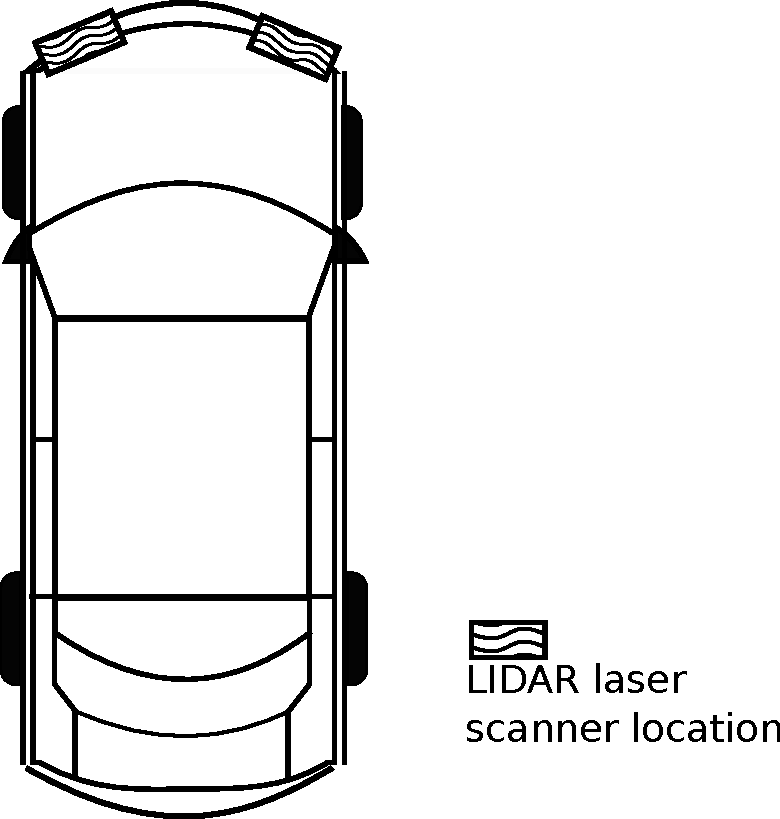
\includegraphics[scale=0.4]{img/fig:demonstrator:birdeye}
     \end{tabular}
   \caption{Bird-eye view: LIDAR laser scanners location}
   \label{fig:demonstrator:birdeye}
\end{figure}

Each LIDAR is distributed in layers (Figure~\ref{fig:demonstrator:lateral}) and scanning range (Figure~\ref{fig:demonstrator:superior}). 

There are four layers in total, each layer disposed vertically in different angles. The road is considered as base for the angle formation. This angle is formed by an imaginary line, which is parallel to the road surface, and the layer trajectory. Those angles are depicted in the Figure~\ref{fig:demonstrator:lateral}.

\begin{figure}[h]
   \centering
     \begin{tabular}{lr}
       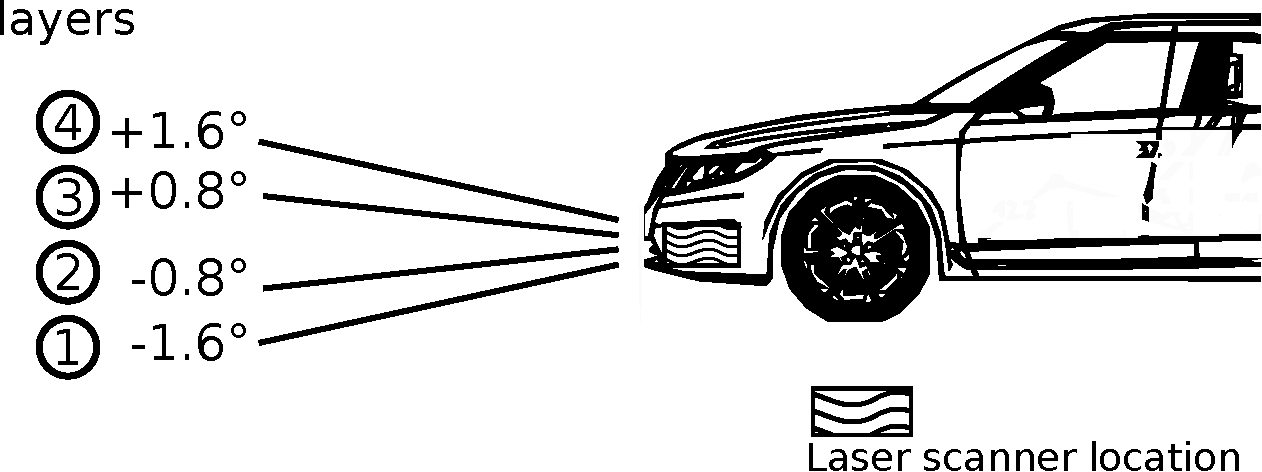
\includegraphics[scale=0.5]{img/fig:demonstrator:lateral}
     \end{tabular}
   \caption{Lateral view: Four layers of the left LIDAR laser scanner}
   \label{fig:demonstrator:lateral}
\end{figure}

A single layer sweeps the environment in a limited range, in the Table~\ref{tab:beam:interception} we can see the layers and their specific range. The LIDAR laser scanner used in our tests have the $0.5^{\circ}$ resolution, meaning that every layer is capable of collecting samples at $0.5^{\circ}$ of distance in between. 

To calculate the number of beams available in the layer $\ell$, we apply the Equation~\ref{eq:totalbeams}, where the functions $min$ and $max$ are the minimum and maximum angles that can be reached by the layer $\ell$, and the function $resolution$ gives the resolution of the LIDAR laser scanner $\rho$, this specification is provided by the manufacturer. 

Thus, we can calculate the number of beams in a layer according with its range. Let's take as example the first layer and calculate the number of beans available in this layer. 

The first layer has a range that varies from $+35^\circ$ to $-60^\circ$ (minimum and maximum range, respectively), the resolution is $0.5^\circ$, according to the specification of the manufacturer. By applying those values in the Equation~\ref{eq:totalbeams} we have $190$ beams available for the first layer.

\begin{equation}
\label{eq:totalbeams}
beams_{total}(\ell)=\frac{|max(\ell)-min(\ell)|}{resolution(\rho)}
\end{equation}


From every individual beam is possible to obtain the \textit{impact point}, meaning the distance between the LIDAR laser scanner and the first object to intercept the laser beam.

\begin{figure}[h]
   \centering
     \begin{tabular}{lr}
       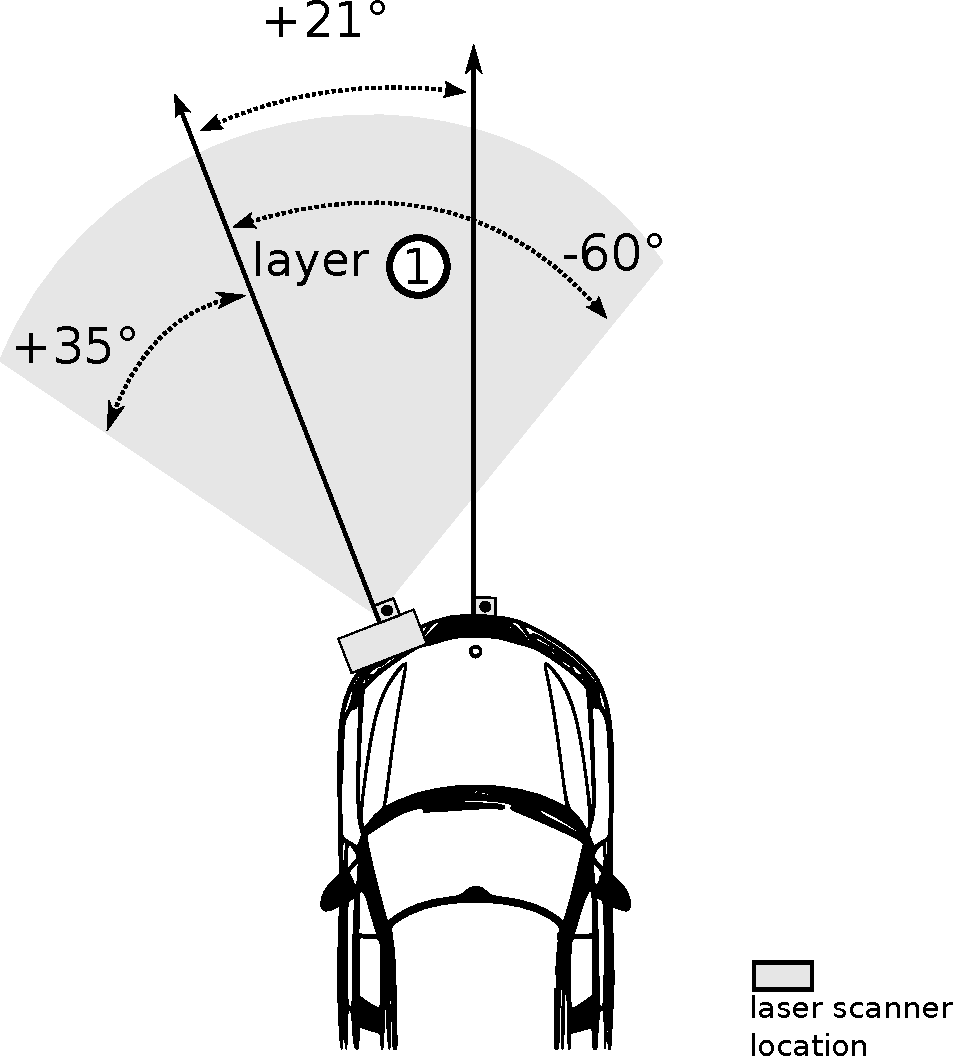
\includegraphics[scale=0.5]{img/fig:demonstrator:superior}
     \end{tabular}
   \caption{Bird-eye view: Left LIDAR laser scanner range, for the first layer}
   \label{fig:demonstrator:superior}
\end{figure}


\begin{table}
\label{tab:beam:interception}
	\begin{center}
	    \begin{tabular}{ | c | c | c | c | c |}
		    \hline
		    Layer & $+50^\circ$ & $+35^\circ$ & $-50^\circ$ & $-60^\circ$ \\ \hline
		    4 & + & + & + &  \\ \hline
		    3 & + & + & + &  \\ \hline
		    2 &  & + & + & + \\ \hline
		    1 &  & + & + & + \\ \hline
		    $\cap$ &  & + & + &  \\ \hline
	    \end{tabular}
	\end{center}
    \caption{Layers and the horizontal distribution of the beams}
\end{table}

The testbed has two LIDAR installed, the multiple sensor usage in the demonstrator car makes of it a complex system, due to the number of data gathered, overlapped information and possible conflicted data. Thus, all sensor information must be carried in a consistent manner and this is accomplished by fusing the sensor information, more details about how this is done in the Section~\ref{sec:sensor:fusion}.

\section{Sensor pre-processing} %fusion module
\label{sec:sensor:fusion}

% in the last subsection, output form (occupancy grid), digrams; explains that this is our input

\subsection{Purpose}

The demonstrator car is composed with two LIDAR laser scanner sensors, as we saw in the Section~\ref{sec:sensor:fusion}. Each of the LIDAR laser scanner is composed of few layers and each layer contains several beams. Those beams are spread horizontally in a given angle range, the ranging (initial and final angles) depends on the layer.

\begin{figure}[h]
   \centering
     \begin{tabular}{lr}
       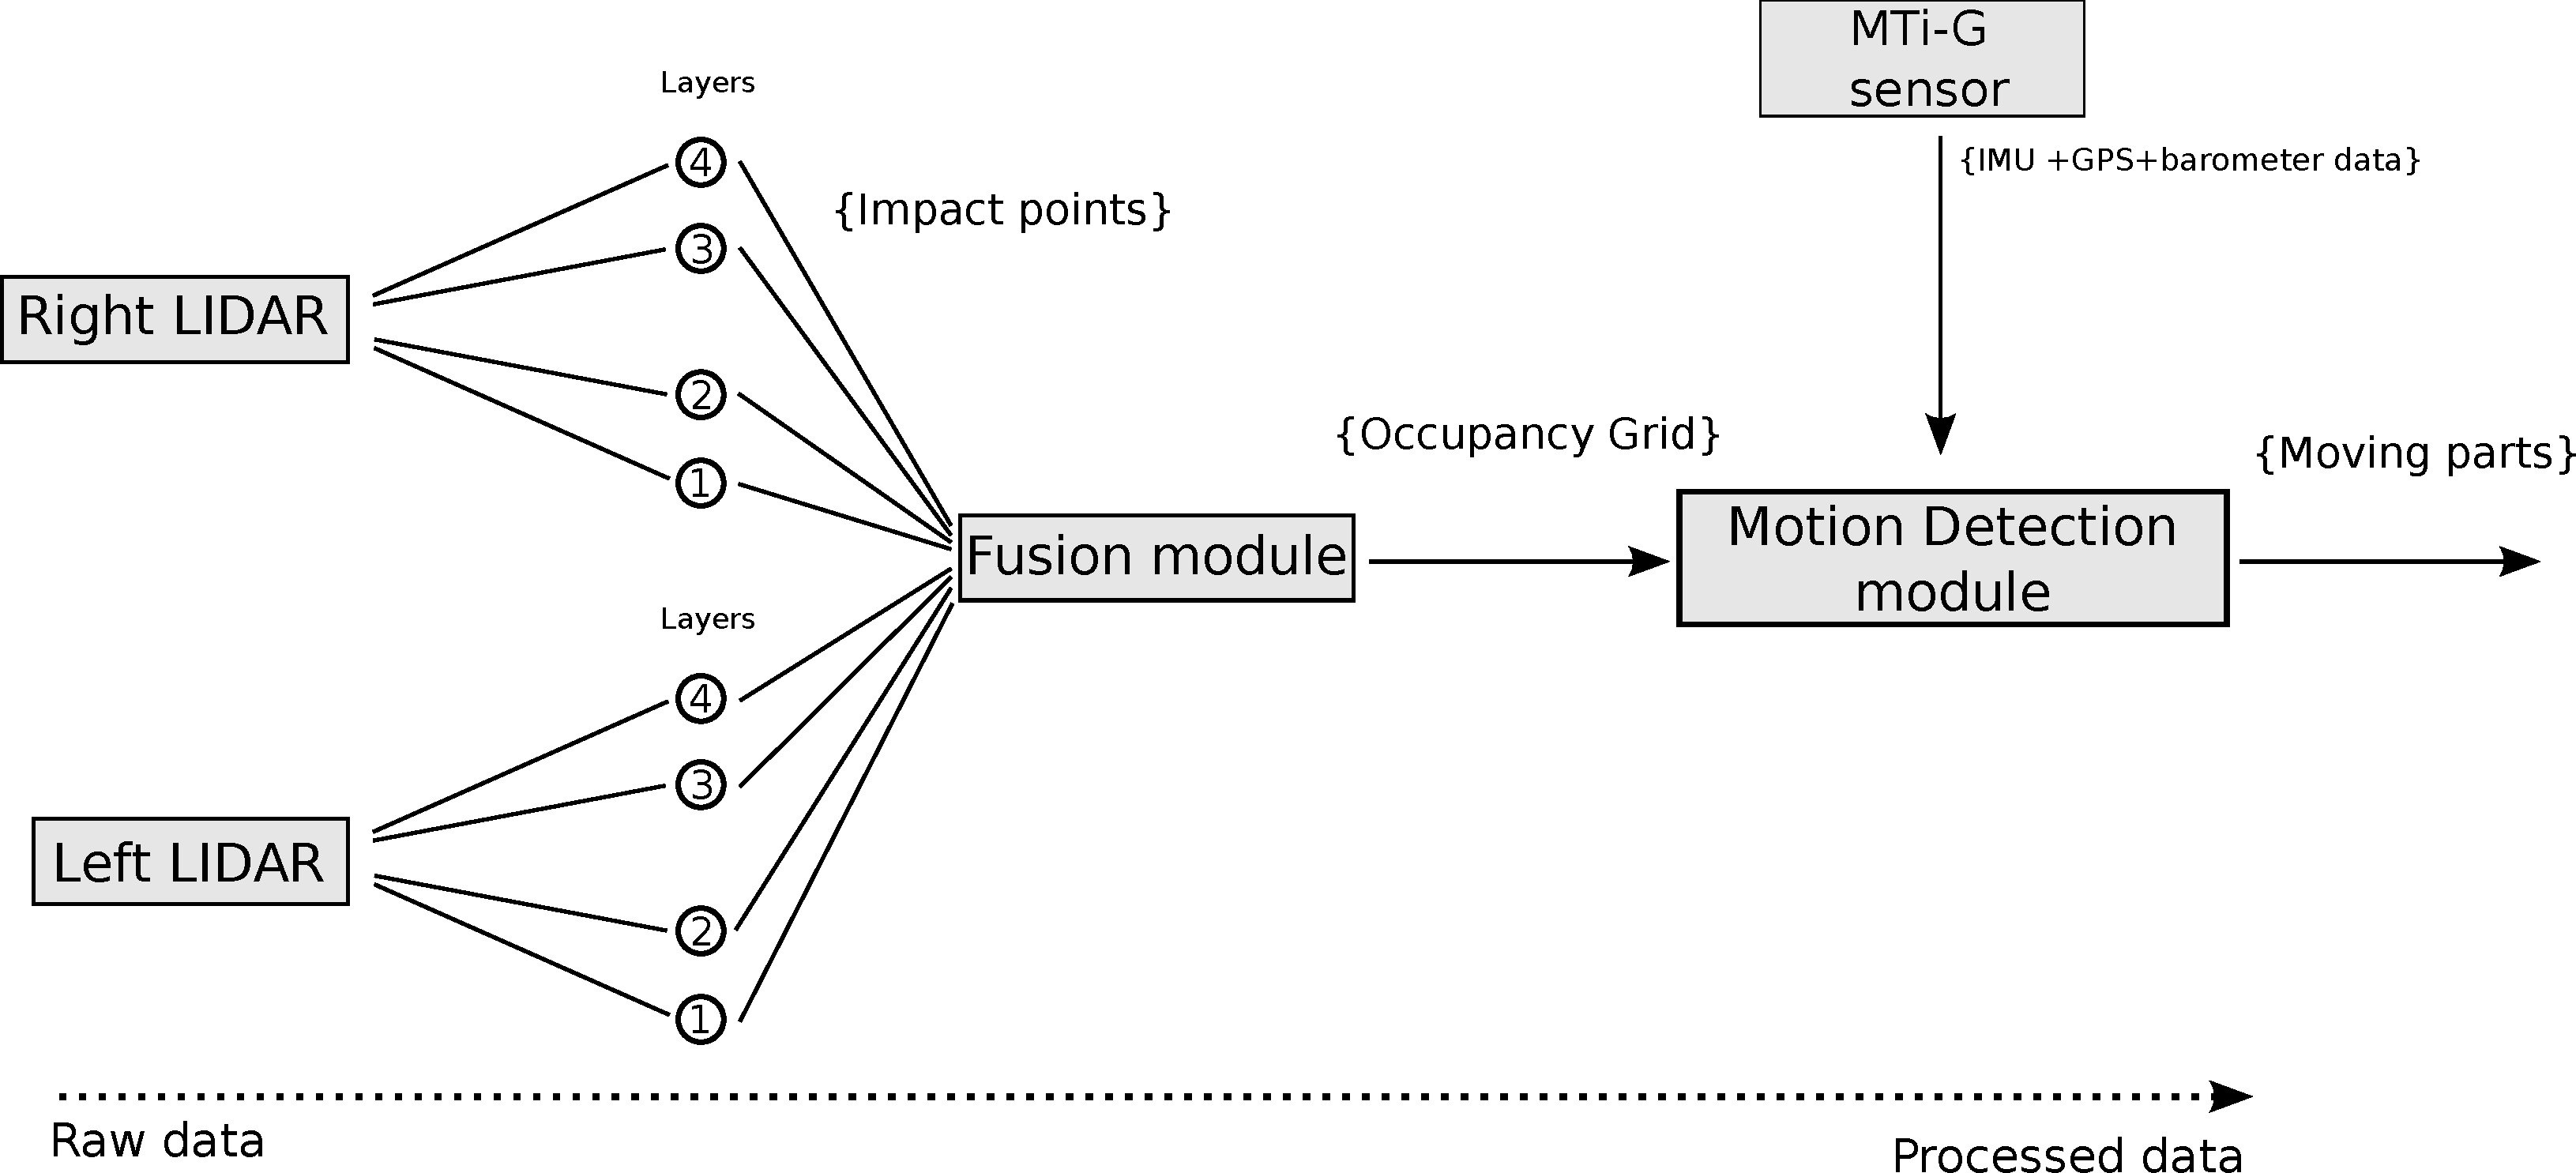
\includegraphics[scale=0.30]{img/fig:motion:framework}
     \end{tabular}
   \caption{General framework for moving objects detection}
   \label{fig:motion:framework}
\end{figure}

This data must be gathered together, but how give a unique representation for all information provided by the sensors in one single visualization? Recall that there are overlapping scanner reading, which means that there may exist conflicting readings due to the sensor failure.

To solve that issue, the data of the different layers are fused. The technique adopted for the fusion was \textit{Linear Opinion Pools}, which results in the Occupancy Grid with fused data\cite{ADARVE-2012-671211}.

\subsection{Building the Occupancy Grid}


\subsubsection{The Grid}
\label{ch03:buildgrid:grid}

In a grid, the space interacting with the robot (the car demonstrator in our case) is discretized in regular sized independent cells, just like the one depicted in the Section~\ref{ch02:gridbased}.

If we plot the output data from the LIDAR laser scanner sensors in an image, it will be similar to Figure~\ref{fig:motion:impactpoint}, which is the representation of the impact points. This representation suffer from two problems:

\begin{itemize}
\item singular sensing
\item oblivious blind spot 
\end{itemize}

\textbf{Singular sensing} meaning that this representation presents information obtained by only one layer, although the LIDAR provides several layers with overlapping spots, which can help reduce the uncertainty of the sensors in some areas of the image. 

\begin{figure}[h]
   \centering
     \begin{tabular}{lr}
       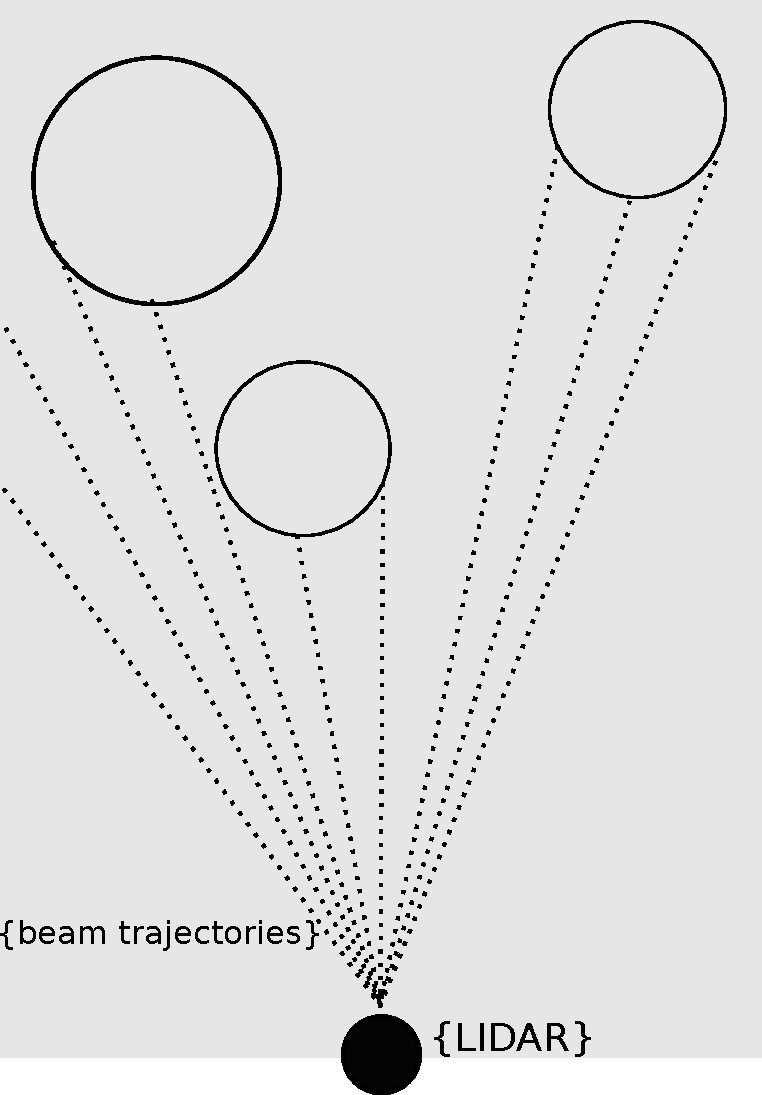
\includegraphics[width=0.3\columnwidth]{img/fig:motion:impactpoint:01}
       & 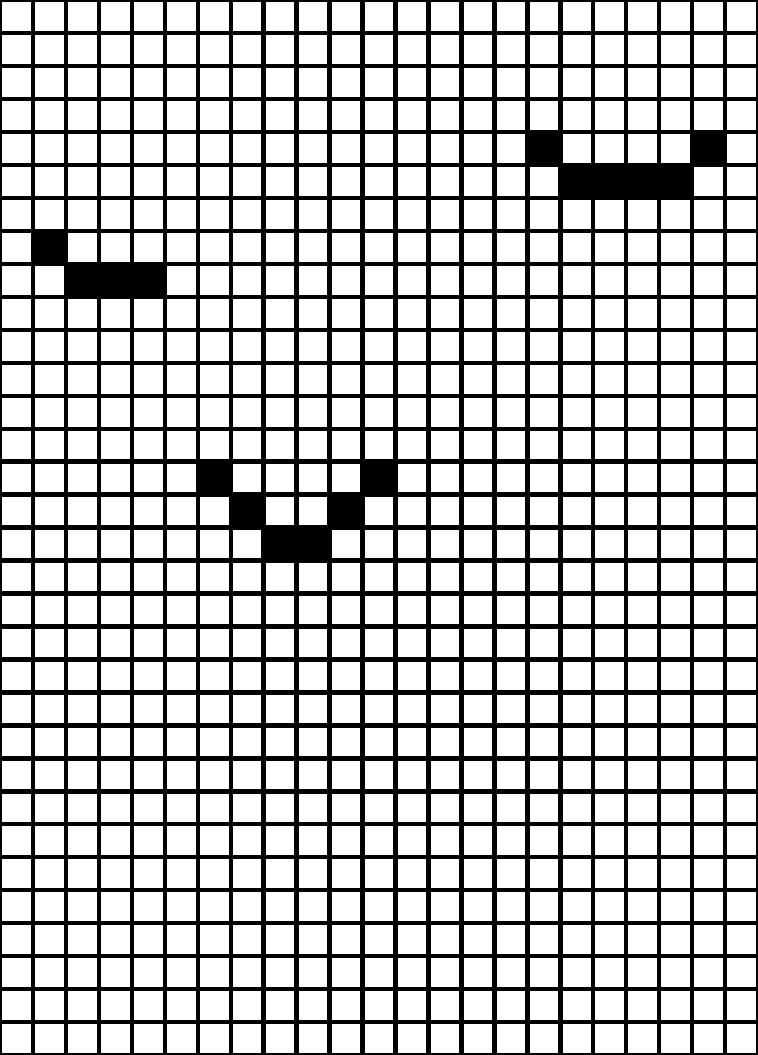
\includegraphics[width=0.3\columnwidth]{img/fig:motion:impactpoint:02}
     \end{tabular}
   \caption{LIDAR laser scanner and impact points: On left the real environment \& On the right side the grid with impact point}
   \label{fig:motion:impactpoint}
 \end{figure}


\textbf{Oblivious blind spot} happens due to missing information about some cells, nothing is said about the other regions of the environment other than the impact points. We must to have a complete, or at least as complete as possible, representation of the environment even for those spots that are not observed by the sensor. In the Figure~\ref{fig:motion:impactpoint}, we can observe that there is no information about spots locate right after the impact point.

Based in the work \cite{ADARVE-2012-671211} we can build a grid which contains the occupancy probability for all cells in the map for LIDAR laser scanner.

For that we need to make the fusion of the layers($\ell$) provided by LIDAR. In the Equation~\ref{eq:sensor:lidarfusion} we want calculate the values for every individual cell. For given cell $C$, the probability of having this cell occupied is calculated with the agreement of all layers provided by the LIDAR.

\begin{equation}
\label{eq:sensor:lidarfusion}
P(C|\ell_1,\ell_2,\ell_3,\ell_4)
\end{equation}

Assuming we want to generate the occupancy grid for an space of $NxM$ cells, this would be calculated according to the Equation~\ref{eq:sensor:gridcalculation}. The Equation~\ref{eq:sensor:gridcalculation} take into consideration a confidence weight $w(C)$ for the measure obtained for the cell $C$ and the probability that the cell is occupied $P(C|\ell_i)$.

\begin{equation}
\label{eq:sensor:gridcalculation}
P(C|\ell_1,\ell_2,\ell_3,\ell_4)=\alpha \sum_{i=1}^{4} w_i(C)P(C|\ell_i)
\end{equation}

The calculation of the cell occupancy is made differently depending on two situations. Depending on the position of the cell $C$ relative to the impact point.

If the cell $C$ is located before an impact point (in between the LIDAR and impact point), the occupancy of that cell is calculated in function of the distance between the cell and the impact point, due to the uncertainty of the sensor model the normal distribution function $\eta$ is taken into consideration\cite{iyengar1991autonomous} Equation~\ref{eq:sensor:normal}.

If the cell $C$ is located after the impact point, the probability assigned to the cell will be $max(0.5;d(p_c,p_l))$.

\begin{equation}
\label{eq:sensor:normal}
\eta(x;\mu,\sigma)=\frac{1}{\sigma \sqrt{2\pi}}e^{-\frac{1}{2}(\frac{x-\mu}{\sigma})^2} 
\end{equation}

The function $w(C)$, which is the confidence of the value measured, has two components: the probability of an \textbf{unexpected object} to appear and the \textbf{angle} of the beam with respect to the road.

\paragraph*{Beam hit angle} the angle formed between the beam (from LIDAR laser scanner) and the road can determine the maximum distance in which the beam can reach. By determining this factor we can establish the confidence of the beam in function of its maximum distance. By that we reduce the reliability of the impact points if it happen beyond the this \textit{maxima}. 

This confidence is calculated according to the Equation~\ref{eq:sensor:confidence:angle}. In which the $z$ represents the distance between the target cell for the calculation and the LIDAR, the angle of the beam $\phi$ and the height of the LIDAR $h_l$ are parameters to calculate the maximum distance of the beam. 

\begin{equation}
\label{eq:sensor:confidence:angle}
C_{angle}=max\{1+\frac{z\tan{\phi}}{h_l},0\}
\end{equation}

\paragraph*{Unexpected object} the probability of an unexpected object to appear is modeled with exponential distribution and normal distribution. If the cell located before the impact point it is modeled with exponential distribution, otherwise the normal normal $\eta$ distribution is used. The canonical form for the exponential distribution is given in the Equation~\ref{eq:sensor:confidence:uo:ed}

\begin{equation}
\label{eq:sensor:confidence:uo:ed}
C_{unexpect}=\lambda e^{\lambda \xi}
\end{equation}

\paragraph*{Confidence composition} is done by gathering the Equations~\ref{eq:sensor:confidence:angle} and ~\ref{eq:sensor:confidence:uo:ed}.

\begin{equation}
C_{total}=C_{total}\ x\ C_{unexpect}
\end{equation}

\subsubsection{Justifying the performance}

The independence among the cells is the main responsible for the high level of parallelism in the algorithm, the high level of parallelism and the performance can be assured by \textit{Amidahls law}.

\textit{Amidahls law} is a diminishing return law. It states that the gaining in performance (speedup) is not necessarily in the same magnitude as the number of new workers added for the execution of the algorithm\cite{Amdahl:1967:VSP:1465482.1465560}. This is pretty much saying that one adult female can have one children in 9 months but two adult female cannot have one children in 4.5 months, it always depends if the task can be really be accomplished in parallel, of course this is an simplistic view, but gives you an idea.

In the Equation~\ref{eq:amidahls}, Amidahls describes the time to execute an algorithm in parallel ($T_p$). Its execution time depends on the time required by sequential part of the algorithm ($T_{seq}$, part which can not be parallel) along with the time for part of the algorithm that can be parallel($T_{par}$) divided by the number of workers ($p$, \textit{e.g.} number of cores in a multi-core processor).

\begin{equation}
\label{eq:amidahls}
T_p=T_{seq}+{T_{par} \over p}
\end{equation}

As in our case the cells are completely independent, the gaining in parallelization is maximum since the term $T_{seq}$ is zero (the sequential code is inexistent), and the processing time is divided among the workers.

\section{The algorithm}
%motion detection

\subsection{Principle} 

\textit{Frame} is a snapshot of the current environment representation, it is used as one of the inputs required for the algorithm developed in this work. This algorithm requires the minimum amount of two \textit{frames} to work. 

But before jump on explanations on how those two frames are going to be used, we need to describe how those frames are obtained and how they mimic the environment.

In the Section~\ref{sec:demonstrator}, we saw that our test platform is composed by two scanners, each of them containing several layers. Every layer has a certain number of beams, which are spread horizontally within a regular angle interval. 

So, before having a frame that can be used by our algorithm, its required to perform the fusion of the layers from the LIDAR, which is done by the \textbf{Fusion module}. 

The details about the techniques adopted and the data processing were explained in the Section~\ref{ch03:buildgrid:grid}. From here on, we are going to proceed with explanation of our methods, which is identified as \textbf{Motion detection module}. This module is located at the end of the processing chain, as exhibit in the Figure~\ref{fig:motion:framework}. 

\begin{figure}[h]
   \centering
     \begin{tabular}{lr}
       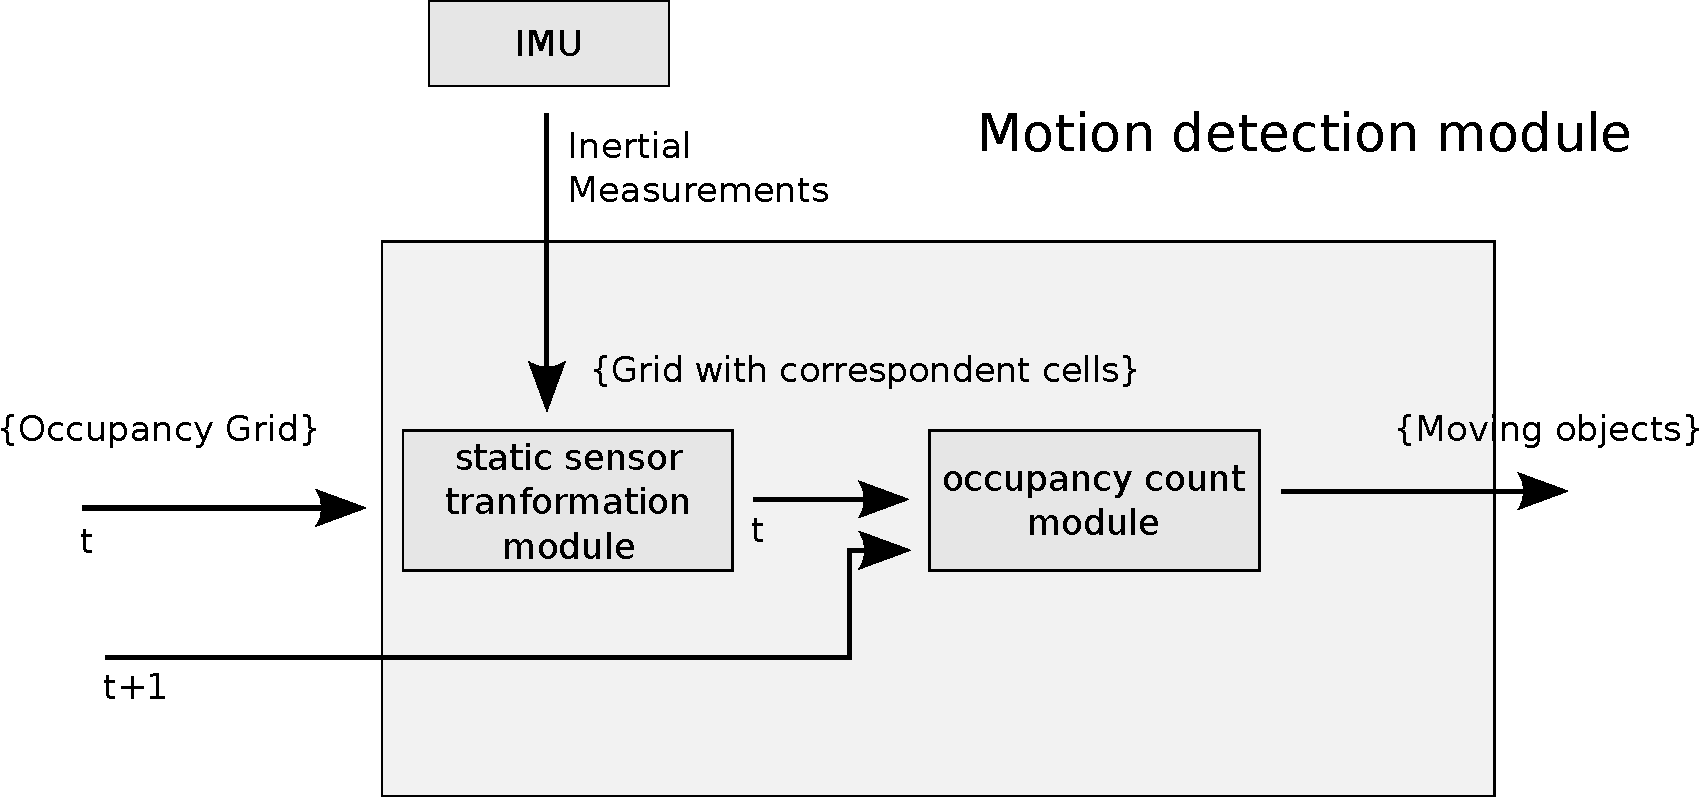
\includegraphics[scale=0.50]{img/fig:motion:framework:motionmodule}
     \end{tabular}
   \caption{Motion detection module anatomy}
   \label{fig:motion:framework:motionmodule}
\end{figure}



\subsection{Non-static sensor issue}

The LIDAR is installed on a vehicle, the goal is to acquire measures while vehicle is moving. So it captures the surrounding and the data is processed by the \textbf{fusion module} resulting in Occupancy Grid $OG_t$. This process is repeated for each frame obtained. This is required to transform the data into the proper input required by the \textbf{motion detection module}.

The position of the LIDAR gives us the fully dynamic scenario impression. Meaning that, by the LIDAR sensor perspective the entire scenario is moving and all subjects are changing their position, except for those who are following the same trajectory as the vehicle and at the speed. 

The footage used in the tests are recorded in $24fps$ (frames per second). Although we have a large amount of frames in a sequence we are able to achieve good qualitative results by using two frames. 

Due to the good qualitative results obtained by using the two frames approach, we will demonstrate all formulas by considering such configuration - only two frames for the calculation. But we may reference other frames in situational examples.


\begin{figure}[h]
   \centering
     \begin{tabular}{lr}
       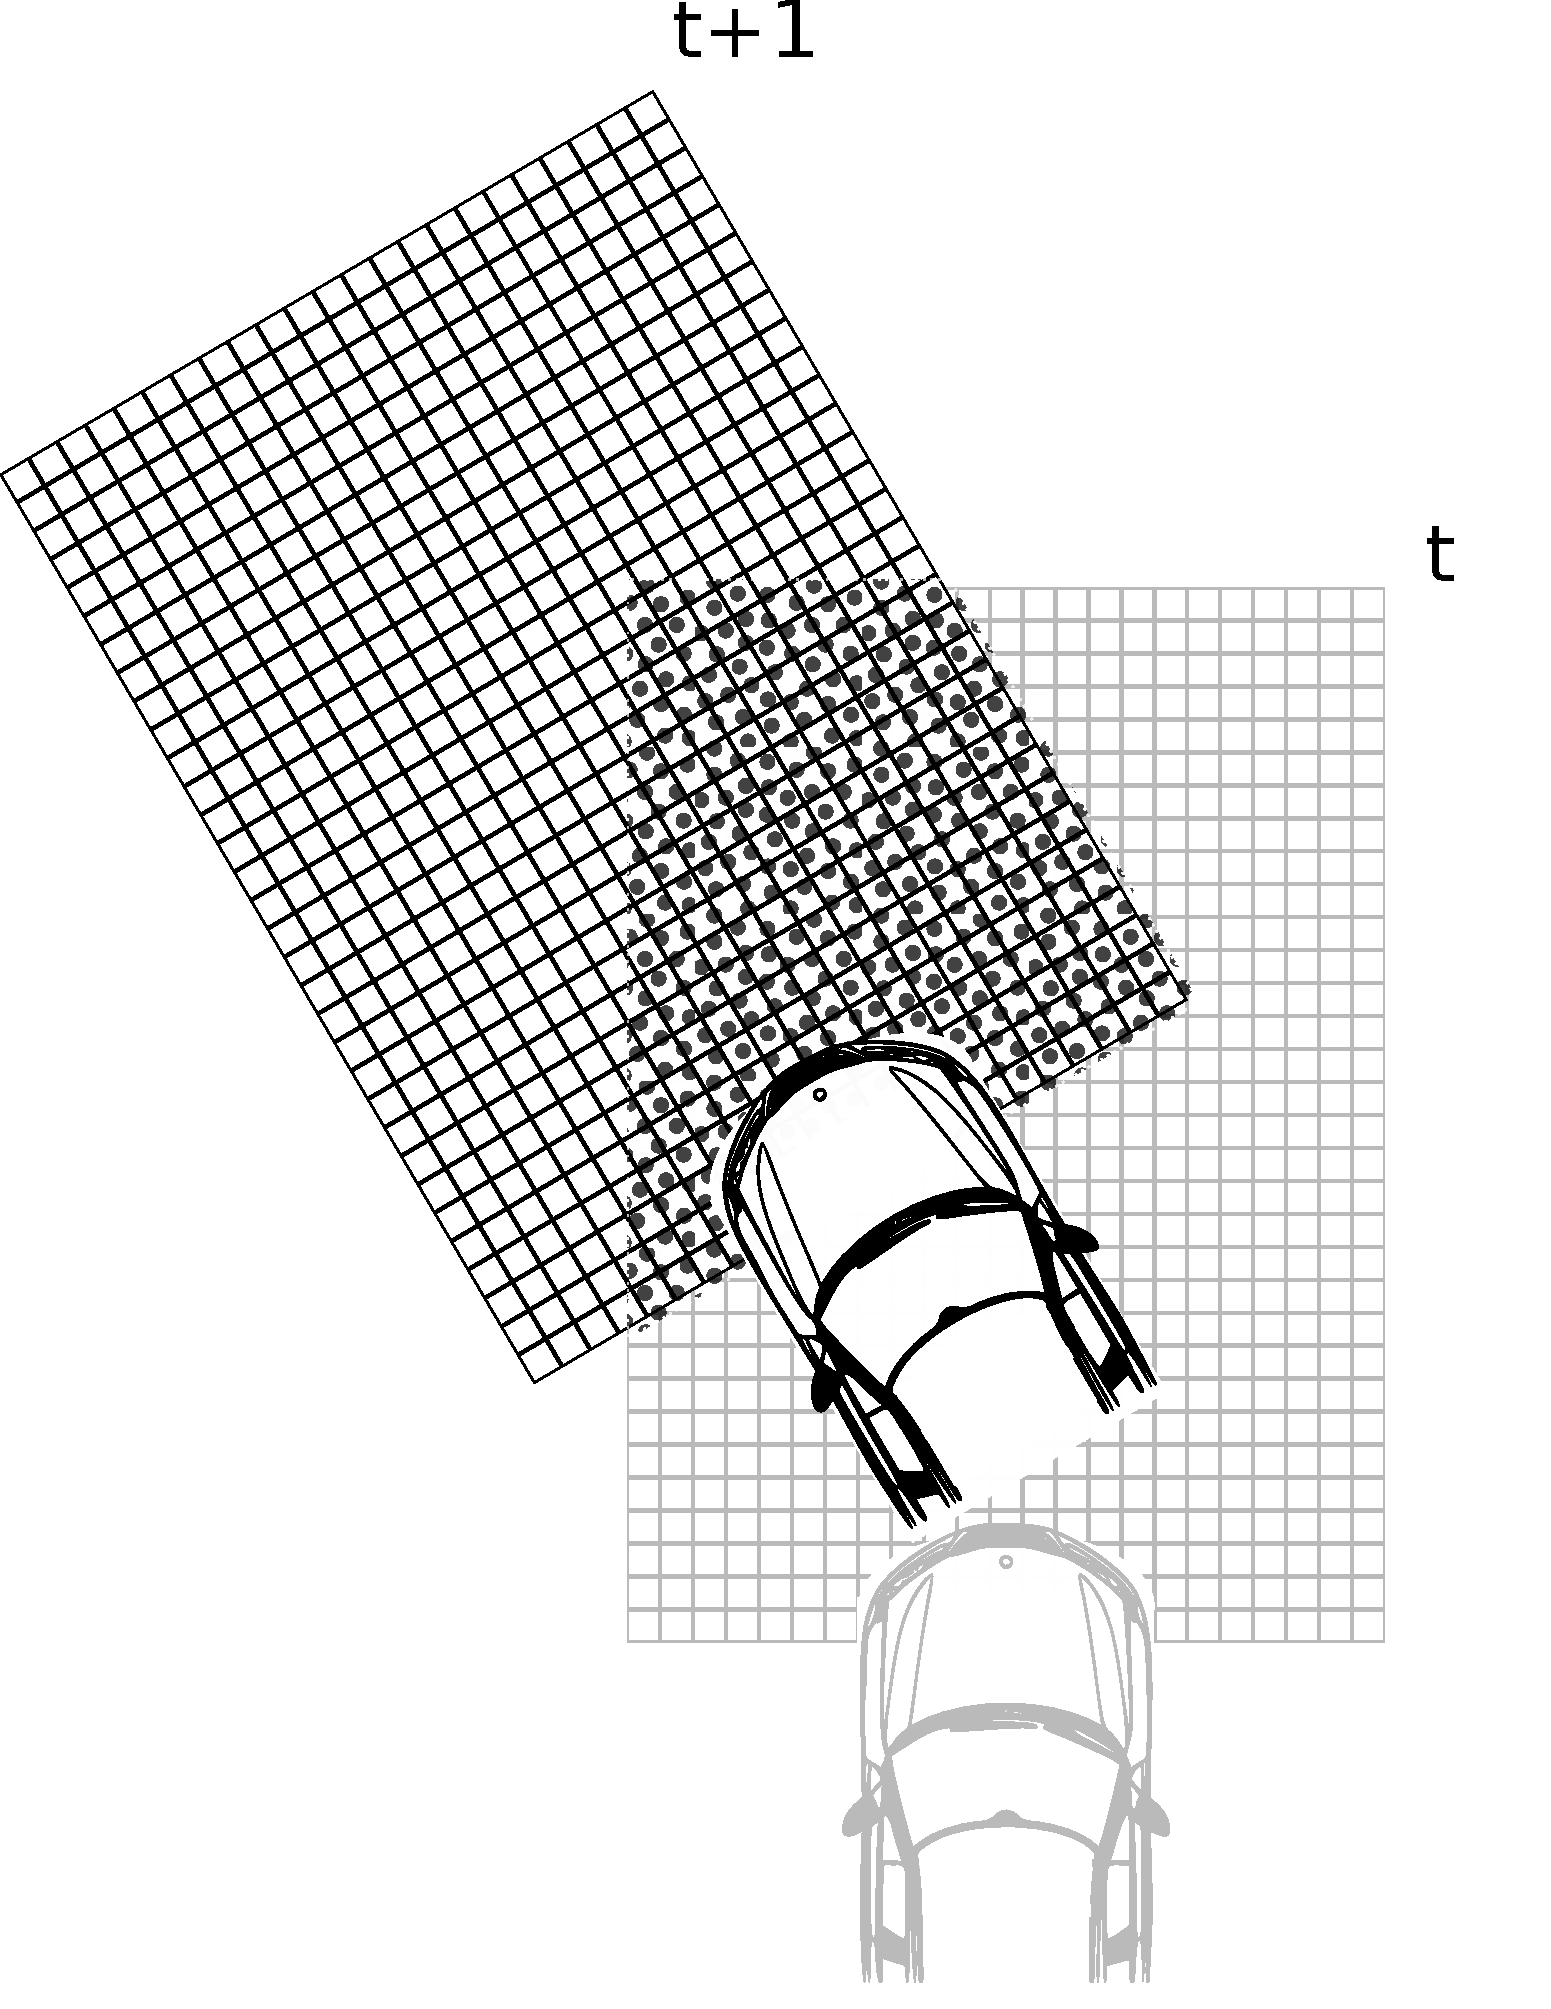
\includegraphics[width=0.35\columnwidth]{img/fig:motion:algorithm:nonstatic:01}
       & 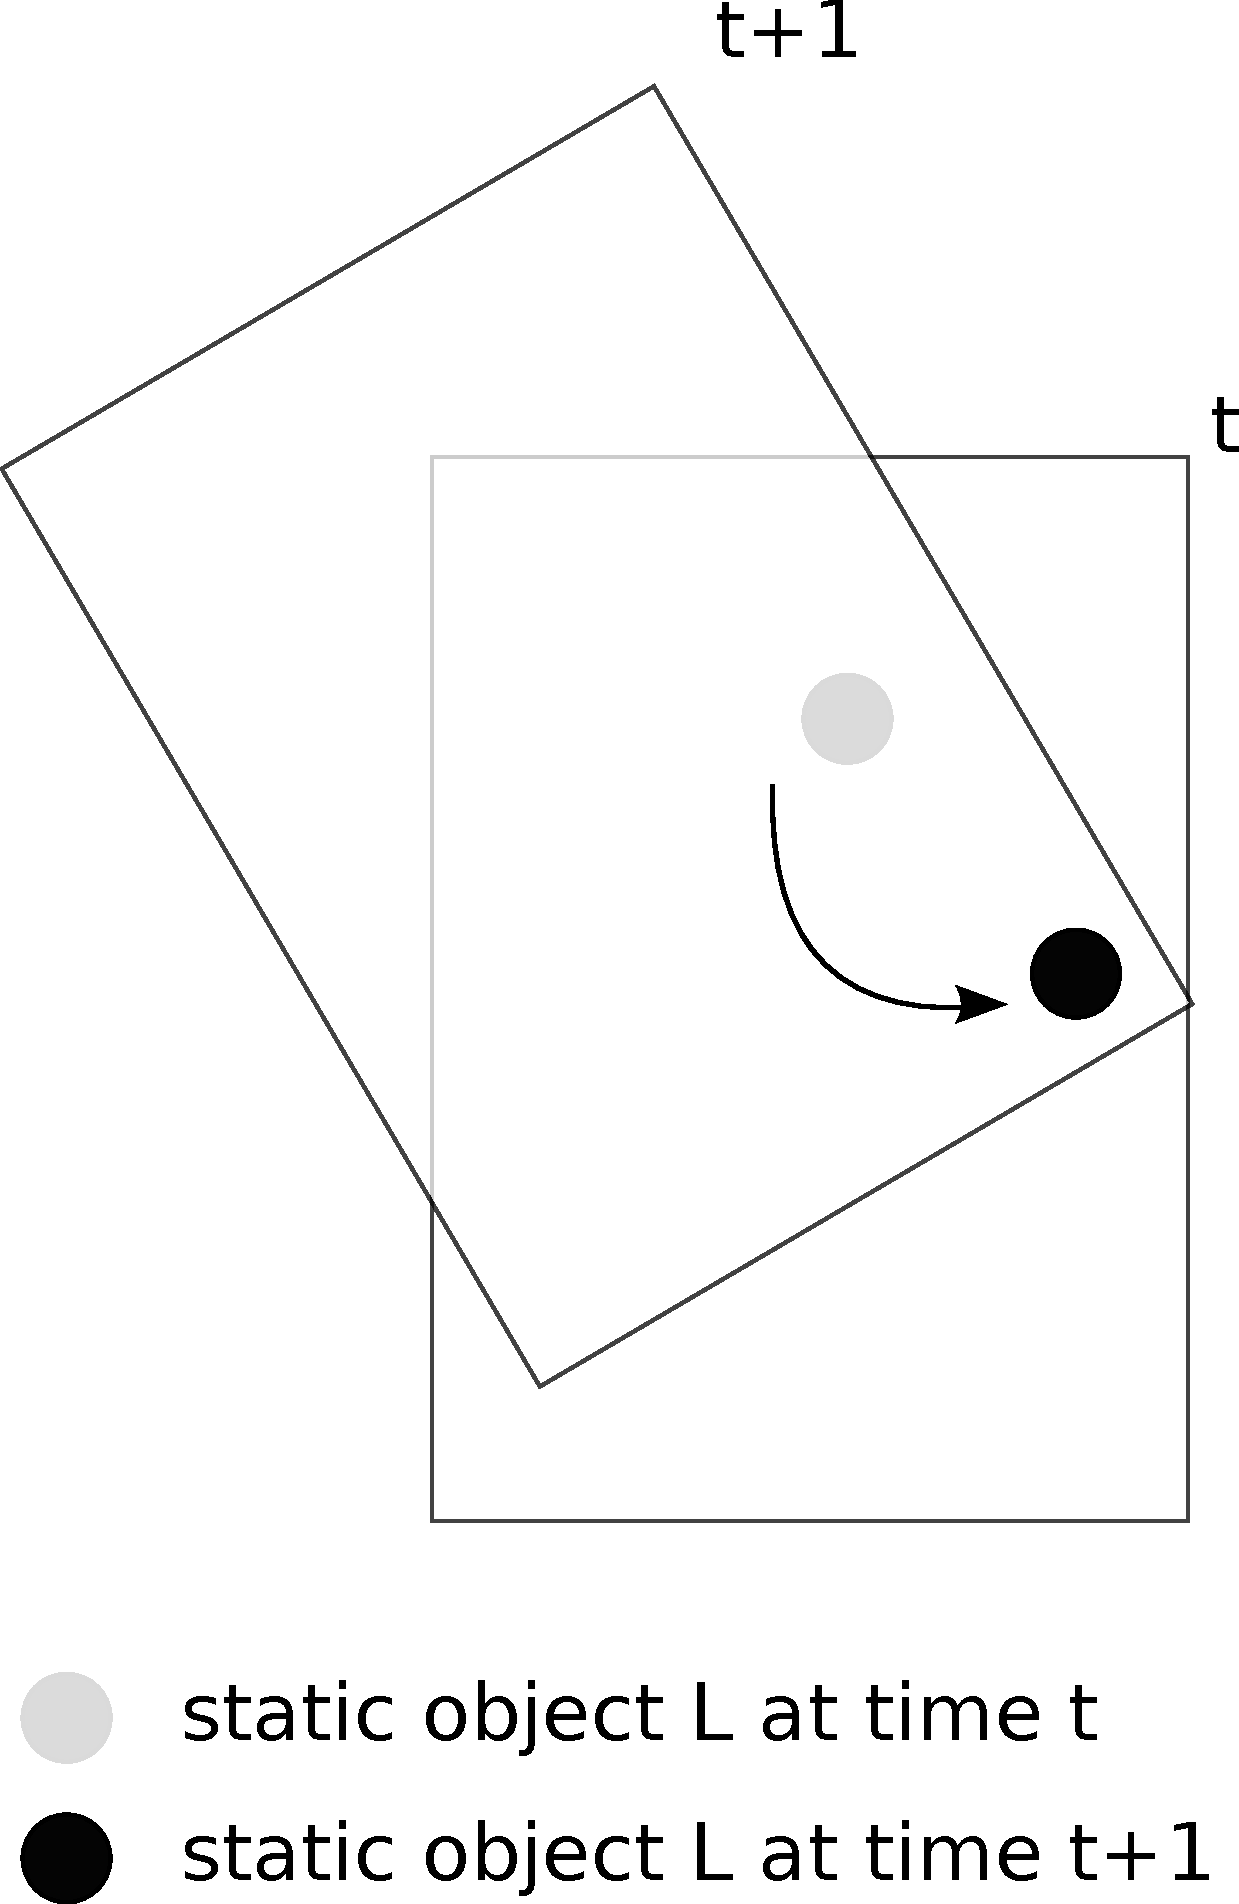
\includegraphics[width=0.3\columnwidth]{img/fig:motion:algorithm:nonstatic:02}
     \end{tabular}
   \caption{frames $f_t$ and $f_{t+1}$ with the intersection area}
   \label{fig:motion:algorithm:nonstatic:01}
 \end{figure}

The method developed in this document requires the static sensor constraint, this constraint assumes that there is an exact correspondence between the cells among the two frames analyzed. Such constraint is not true in our application since the goal is to have it running in a moving care, as an ADAS application. 

To better understand this issue take a look at the example: assume our vehicle is driving along a street and makes a left turn, we capture two frames, one while the car was driving straight $f_t$, and the second frame  after the car initiate the left turn $f_{t+1}$. We observe an a static object in the frame $f_t$ that was located at $d_t$ meters from the car, and in the frame $f_{t+1}$ this very same object will be at $d_t-\Delta d(f_t,f_{t+1})$ and will be slightly moved to the right side (due to the left turn). The function $\Delta d$ returns the distance traveled by the car between the two frames. This behavior can be seen in the Figure~\ref{fig:motion:algorithm:nonstatic:01}, and as we can see, we can consider only as two frames the overlapping area (Figure~\ref{fig:motion:algorithm:nonstatic:01} dotted area in the left image), but since this analysis is done in very small time variation, we have a great portion of overlapping area.

This problem is solved by introducing the Inertial Measurement Unit(IMU) data. The IMU provides information about the inertial behavior of the unit. Although not all information generated by the IMU are needed, the ones used are speed $s$, yaw angle, vertical $v_v$ and horizontal $v_h$ velocity. Those informations are used to apply the necessary transformation to the $f_t$ making its cells match the cells $f_{t+1}$. Thus finding the correspondence between cells of $f_t$ and $f_{t+1}$.

From the IMU information we calculate two parameters: angular velocity and the linear velocity. 

Angular velocity is obtained by finding the angle variation between the frames $f_t$ and $f_{t+1}$, according to the Equation~\ref{eq:angularvelocity}, $\Delta t$ represents the time variation between the frames.

\begin{equation}
\label{eq:angularvelocity}
\omega(f_t,f_{t+1}) = \frac{Yaw_{t+1}-Yaw_t}{\Delta t(f_t,f_{t+1})} 
\end{equation} 

The angular velocity is given in degrees, but the IMU gives us a quaternion for the angle of the vehicle. The quaternion is the most common way to represent angles in 3d world, due to the fast calculations and it solves the gym ball lock problem, which is common for euler angles. Converting the value from quaternion to Euler angles is straightforward by the Equation~\ref{eq:quaternion}.

\begin{equation}
\label{eq:quaternion}
Yaw=atan2(2(q_0 q_3+q_1 q_2),1-2(q_2^2+q_3^2))
\end{equation}

The angular velocity $\omega(f_t,f_{t+1})$ is used to adjust the angle of $f_t$, put this value aside, before apply this transformation to the frame $f_t$ we have to calculate the displacement of the grid.

At this point, we have the information about the proper angle for the frame $f_t$, the next step is to calculate the displacement of the frame. The displacement is calculated based on the actual velocity of the vehicle at the time $t$. 

The IMU keeps the velocity in two components, the horizontal $v_h$ and vertical $v_v$ velocities, and to obtain the actual velocity, we can apply the Equation~\ref{eq:velocity}, which extracts the velocity based on the two components.

\begin{equation}
\label{eq:velocity}
v_t=\sqrt{v_h^2+h_v^2}
\end{equation}

%\subsection{Occupancy counting}

%For the moment, we assume that the LIDAR sensor is statically positioned and observes the environment.

%How to update the probability of an Occupancy grid with 
%In the occupancy counting, 


%\subsection{Solution}


%\section{summary}

%summary